% Chapter Template

\chapter{Ensayos y resultados} % Main chapter title

\label{Chapter4} % Change X to a consecutive number; for referencing this chapter elsewhere, use \ref{ChapterX}
En este capítulo se detallan los ensayos realizados para verificar el correcto funcionamiento del prototipo y el cumplimiento de los requisitos tanto en la etapa digital como en la analógica.
%----------------------------------------------------------------------------------------
%	SECTION 1
%----------------------------------------------------------------------------------------

\section{Banco de pruebas}
Para los ensayos efectuados en laboratorio se montó un banco de pruebas, figura \ref{fig:bancoDePruebas}, constituido por los siguientes elementos:

\begin{itemize}
\item Generador DDS FY6900,
\item Cable BNC-SMA (Canal descarga parcial)
\item Cable BNC-Cocodrilos (Canal senoide de referencia)
\item Computadora portátil. 
\item Puerto serie-USB
\item Prototipo funcional.
\end{itemize}


\begin{figure}[ht]
	\centering
	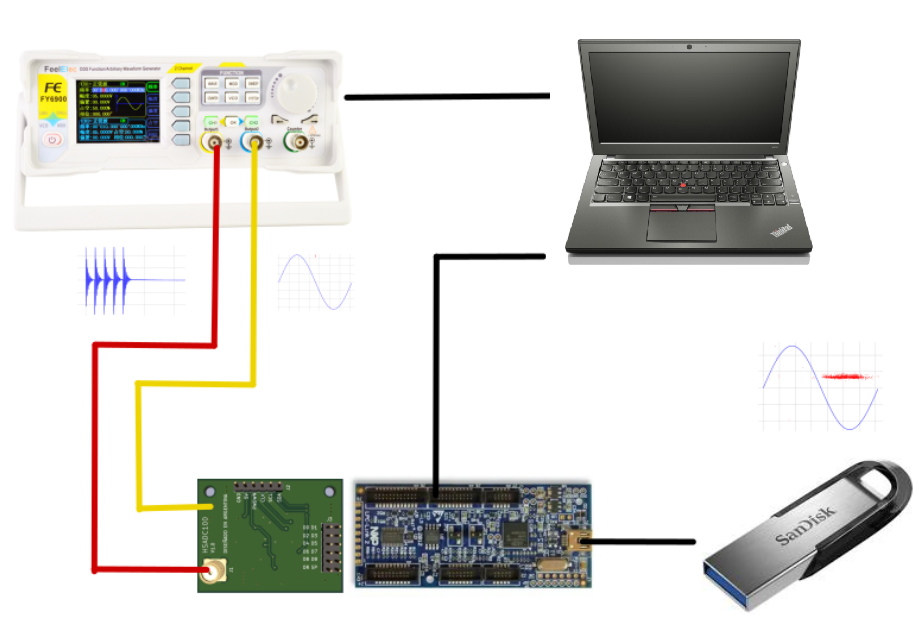
\includegraphics[width=120mm]{./Figures/bancoDePruebas.png}
	\caption{Arquitectura del banco de prueba.}
	\label{fig:bancoDePruebas}
\end{figure}

El banco permitió simular, por medio del generador de señales, la forma de onda de una DP y sincronizarla con una senoide de referencia de 50Hz. La computadora portátil fue utilizada para acceder por medio del puerto serial a la interfaz de usuario del equipo. También se utilizó para controlar al DDS utilizando la base de datos de DP agrupadas por patrones proporcionada por el cliente.
El conjunto de elementos permitió realizar diversas pruebas manuales y automatizadas.

Durante el montaje del banco de pruebas se encontró una limitación en el generador DDS FY6900 que obligó a replantear el proceso de prueba. Debido a que este generador no permite establecer demoras entre los disparo de sus canales las validaciones de amplitud y fase se realizaron en diferentes ensayos.

\section{Ensayos de amplitud}
Durante los ensayos de amplitud se buscó validar que las señales obtenidas por el equipo correspondieran en amplitud y forma con la señales inyectadas por el DDS. Para esto se generaron señales senoidales en diferentes frecuencias y amplitudes.

Este ensayo también se utilizó para validar la respuesta en frecuencia del filtro de entrada. Para esto se inyectaron señales senoidales de 600 mVpp en distintas frecuencias y se realizaron adquisiciones con el fin de comparar lo obtenido con lo inyectado, figura \ref{fig:sin1} y \ref{fig:sin39}. Puede observarse que a igual tensión de entrada, la figura \ref{fig:sin39} se encuentra atenuada en -2,5dB por ser una frecuencia cercana a la frecuencia de corte del filtro. 

\begin{figure}[htpb]
	\hspace{-1.2cm}
	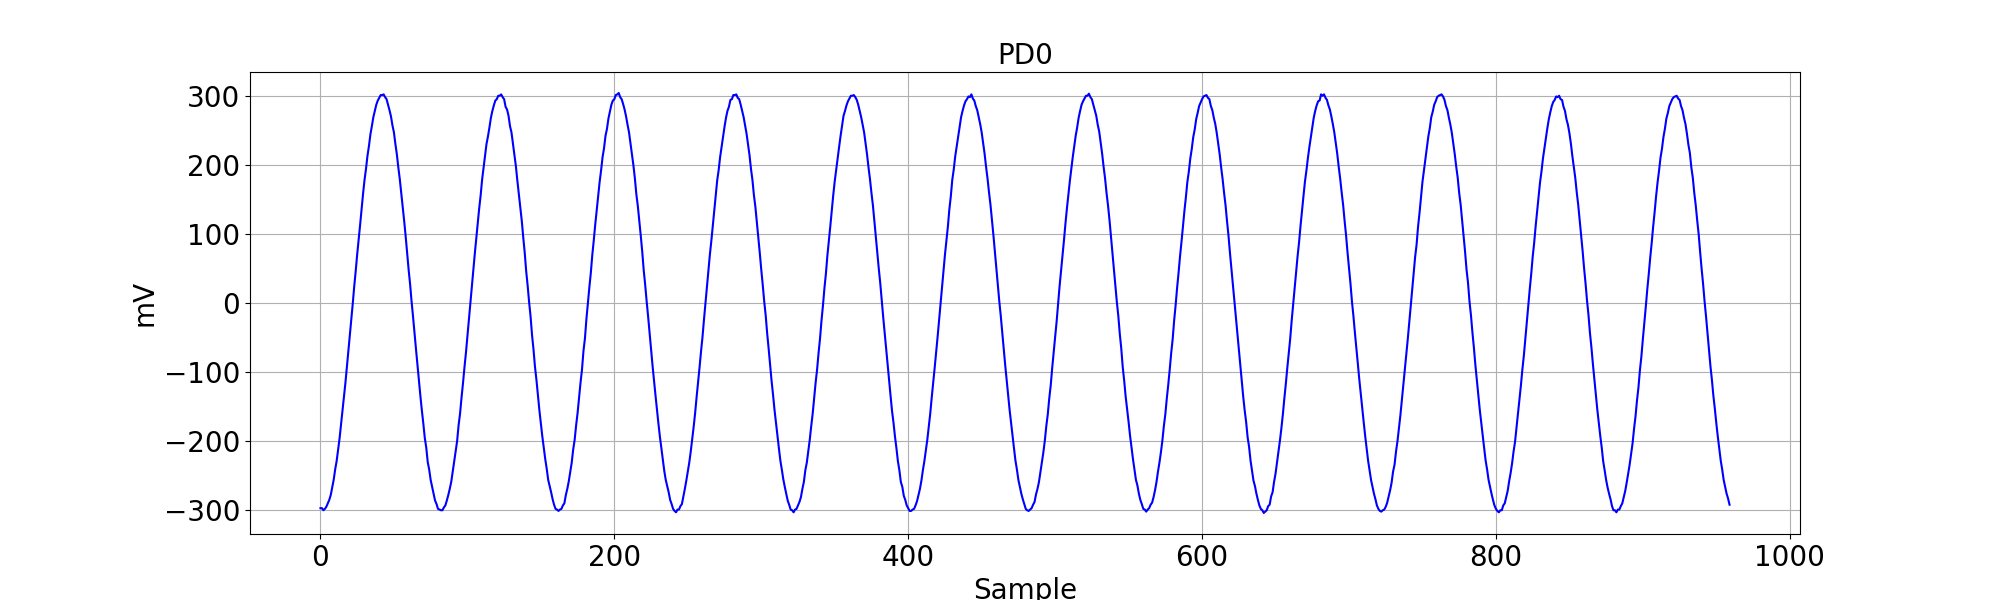
\includegraphics[width=165mm]{./Figures/sin1.png}
	\caption{Señal senoidal adquirida de 1MHz 600 mVpp.}
	\label{fig:sin1}
\end{figure}

\begin{figure}[htpb]
	\hspace{-1.2cm}
	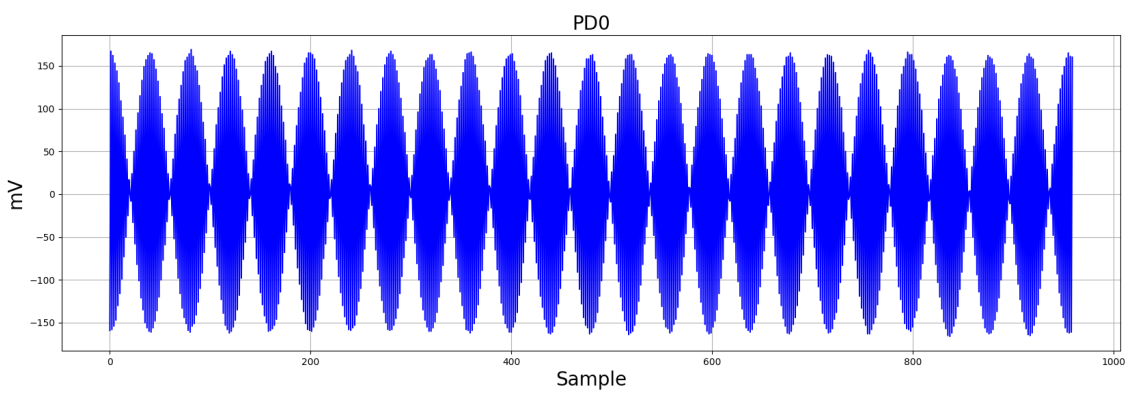
\includegraphics[width=165mm]{./Figures/sin39.png}
	\caption{Señal senoidal adquirida de 39MHz 600 mVpp.}
	\label{fig:sin39}
\end{figure}

\vspace{5mm}

En la tabla \ref{tab:tensiones} se representan la máxima tensión de entrada y la máxima tensión adquirida para cada frecuencia registrada. Por medio de estos valores se calculó la respuesta en frecuencia del filtro real.
 
Para garantizar la correcta detección del valor máximo de la senoide sintetizada, se eligieron frecuencias que no sean múltiplos de la frecuencia de muestreo, de modo de lograr un batido que en un número considerable de muestras se logre barrer un período completo de la señal inyectada.
 
\vspace{5mm}

\begin{table}[h]
\centering
\caption[Antenuación del filtro]{Atenuación del filtro}
\begin{tabular*}{\textwidth}{l c c c c}
\toprule
\textbf{f (MHz)} & \textbf{Entrada (mV)} & \textbf{Salida (mV)} & \textbf{Atenuación (dB)} & \textbf{At. esperada (dB)}\\
\midrule
1 & 600 & 610 & 0,0717 & -0,1770 \\
13 & 600 & 580 & -0,1472 & -0,177 \\
19 & 600 & 540 & -0,4575 & -0,195 \\
25 & 600 & 540 & -0,4575 & -0,237 \\
27 & 600 & 540 & -0,4575 & -0,237 \\
33 & 600 & 520 & -0,6214 & -0,557 \\
39 & 600 & 330 & -2,5963 & -2,265 \\
\bottomrule
\hline
\end{tabular*}
\label{tab:tensiones}
\end{table}

\vspace{5mm}

En la figura \ref{fig:respFrecReal} se puede observar la comparativa entre la respuesta del filtro esperada y la deseada

\vspace{5mm}

\begin{figure}[ht]
	\centering
	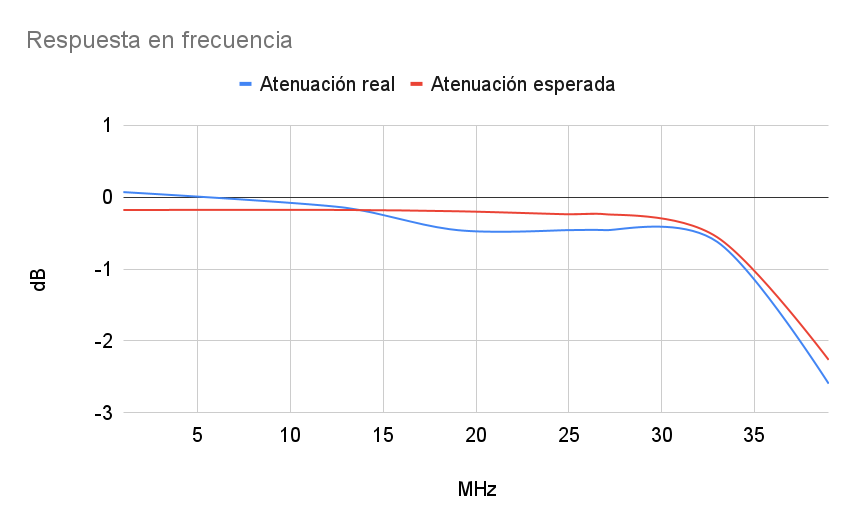
\includegraphics[width=140mm]{./Figures/respFrecReal.png}
	\caption{Respuesta en frecuencia del filtro implementado y su comparación con la respuesta en frecuencia esperada.}
	\label{fig:respFrecReal}
\end{figure}

\vspace{10mm}

\section{Ensayos de integridad}


Durante estos ensayos se buscó determinar que la forma de onda capturada por el prototipo desarrollado sea aceptable y conserve en gran medida la morfología de la señal a adquirir. Para esto se inyectó una DP generada en base a una DP real previamente muestreada, figura \ref{fig:dpSint}.

\vspace{5mm}

\begin{figure}[htpb]
	\hspace{-1.2cm}
	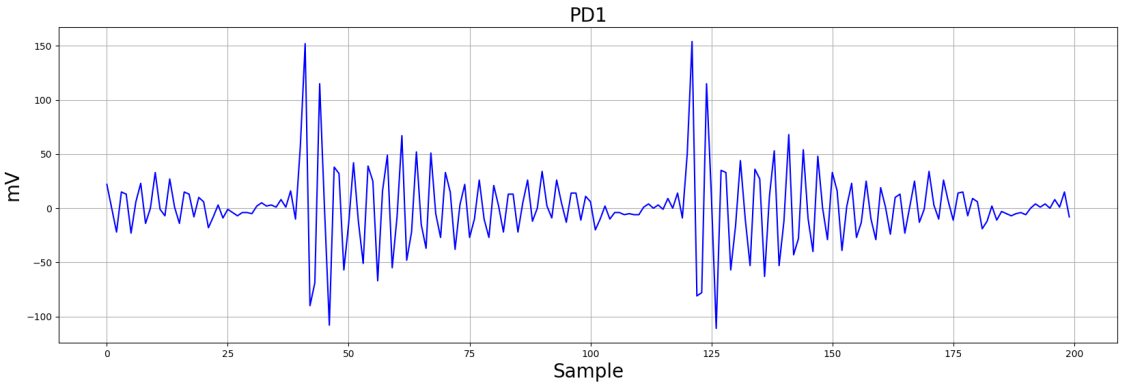
\includegraphics[width=165mm]{./Figures/dpSint.png}
	\caption{DP sintetizada 400mvpp capturada por el equipo.}
	\label{fig:dpSint}
\end{figure}

\vspace{5mm}

La señal generada fue muestreada por medio de un osciloscopio Siglent SDS1202X-E de 200 Mhz de ancho de banda y 1 Gs de tasa de muestreo. La misma señal fue muestreada por el equipo adquisidor de DP a una tasa de 80 Ms. Para que ambas señales tengan las mismas características y puedan ser comparadas, se aplicó de forma matemática sobre la señal muestreada por el osciloscopio la respuesta en frecuencia del filtro que se encuentra en la entrada del equipo. Ambas señales fueron graficadas superpuestas en la figura XX donde se utilizó un trazo continuo azul para las adquisiciones realizadas por el osciloscopio y una serie de puntos en color rojo para las adquisiciones realizadas por el equipo.

Se puede observar que las muestras adquiridas por ambos equipos coinciden para toda la señal. También se identifica una distribución de muestras a 80 M suficiente para detectar el valor máximo sin la necesidad de hacer un \textit{resampling} de la señal.


\vspace{10mm}

\begin{figure}[ht]
	\centering
	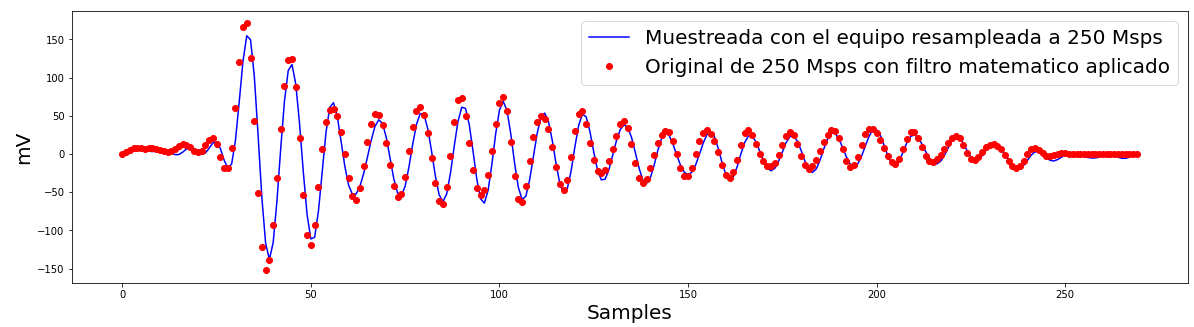
\includegraphics[width=135mm]{./Figures/compPulsos.png}
	\caption{Comparación entre la DP adquirida por el osciloscopio y la DP adquirida adquirida por el equipo.}
	\label{fig:compPulsos}
\end{figure}

\vspace{10mm}

Un análisis de Fourier sobre las señales permitió realizar una comparación de la distribución de energía en el espectro para cada señal, figura \ref{fig:compEspectro}. También se utilizó como herramienta para conocer los componentes principales de frecuencia de la DP analizada.

\begin{figure}[ht]
	\centering
	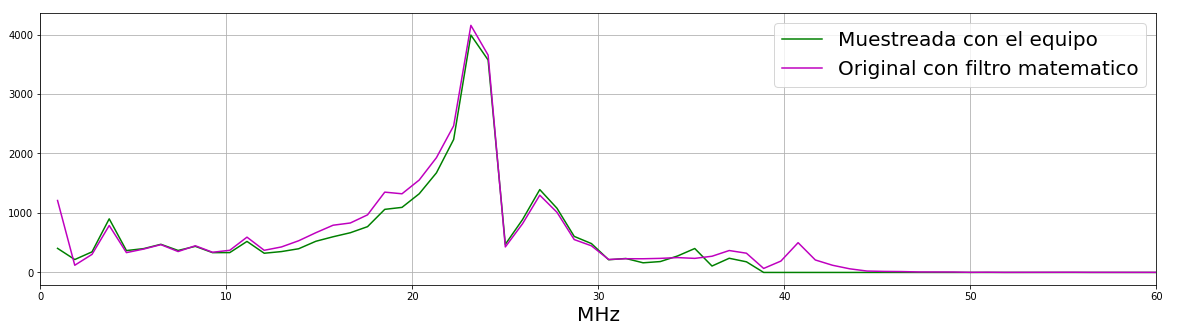
\includegraphics[width=135mm]{./Figures/compEspectro.png}
	\caption{Analisis de Fourier de una DP adquirida por un osciloscopio Siglent SDS1202X-E y  por el equipo.}
	\label{fig:compEspectro}
\end{figure}


\section{Ensayos de disparo}
Durante los ensayos de disparo se realizaron mediciones del tiempo requerido por el sistema para poder rearmar su \textit{trigger}, figura \ref{fig:oscDisparos}. Esta latencia se encuentra determinada principalmente por el tiempo requerido para configurar nuevamente los punteros a memoria y reiniciar el periférico ADC de alta velocidad. 

Durante la adquisición de los \textit{slots} pertenecientes al mismo banco de memoria, el tiempo de rearme fue de 90 uS. Considerando que un grado de la senoide de referencia representa un tiempo igual a 55 uS, la tasa máxima de repetición es de 1 DP cada 1°36’.


\vspace{5mm}

\begin{figure}[ht]
	\centering
	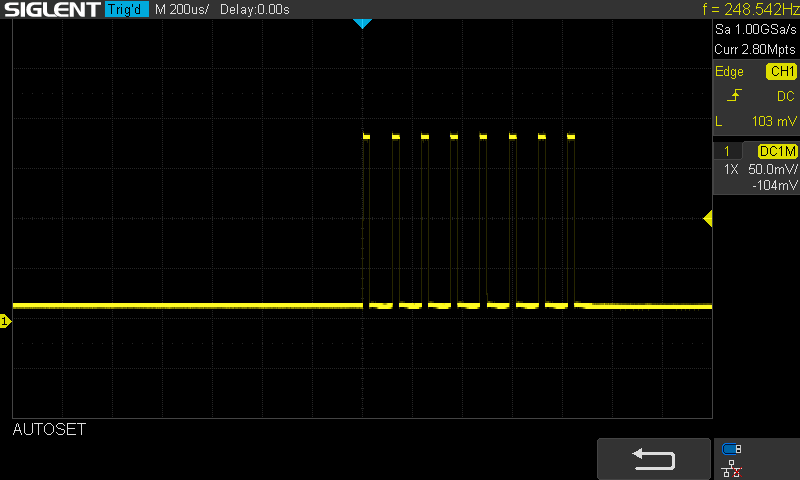
\includegraphics[width=140mm]{./Figures/disparos.png}
	\caption{Adquisición de un banco 16k muestras dividido en 8 slots de 2k muestras cada uno.}
	\label{fig:oscDisparos}
\end{figure}

\vspace{5mm}

\newpage

Además del tiempo requerido para el rearme se realizaron mediciones sobre el tiempo mínimo requerido, por el procesador, para atender el disparo del \textit{trigger}. Este tiempo es de suma importancia porque determina cuantas muestras de desplazamiento existen desde que el \textit{trigger} detectó su disparo hasta que el procesador pudo atenderlo, figuras \ref{fig:tiempoInicial}. 

El tiempo mínimo de latencia para un cortex M4 es de 12 ciclos de reloj. Ya que la velocidad del núcleo es de 204 MHz y la del conversor AD es de 80 MHz se puede determinar que la latencia minima es de 5 muestras. 

Durante esta etapa también se realizaron pruebas comparativas a fin de determinar el \textit{jitter} entre los diferentes disparos. Ya que el tiempo de atención de la interrupción depende ademas de como se haya diseñado el firmware y de la utilización de los bancos de memoria RAM. El \textit{jitter} medido fue siempre inferior a 4 muestras oscilando normalmente entre 1 y 2 .

\vspace{5mm}

\begin{figure}[htpb]
	\hspace{-1.2cm}
	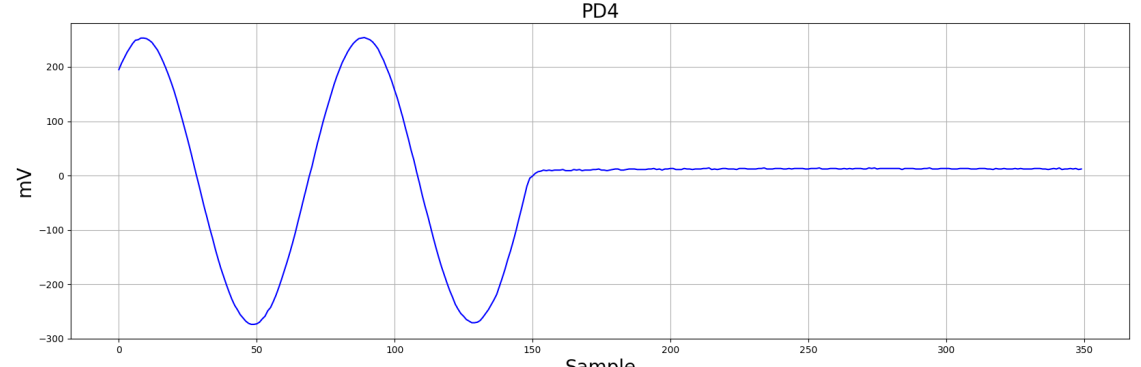
\includegraphics[width=165mm]{./Figures/tiempoInicial.png}
	\caption{Señal senoidal 1 MHz, dos ciclos, trigger 100 mV y flanco ascendente.}
	\label{fig:tiempoInicial}
\end{figure}


\section{Ensayos de fase}

Los ensayos de fase buscan verificar que la detección de una DP determinada está vinculada con el momento angular correcto de la senoide de referencia.

Debido a restricciones del banco de pruebas para disparar una senoide sintetizada de alta frecuencia en un momento angular dado de la senoide de referencia, se recurrió a utilizar una señal cuadrada de 50 Hz con un duty cicle del 0,001\% para la señales positivas y de 99,999\% para las negativas. De esta manera la entrada optoacoplada y la entrada de descargas parciales pudieron ser excitadas en forma conjunta durante todo el periodo de la señal de referencia.

Como consecuencia de este método, la señal inyectada en la entrada de descargas parciales no se encuentra dentro de rango lineal del filtro y es por esto que la medición de tensión no se tomó en cuenta para este ensayo.

La figura \ref{fig:rafagaCero} muestra la adquisición de una serie de pulsos de DP disparados en fase 0 de una senoide de referencia de 50 Hz.

\vspace{5mm}

\begin{figure}[ht]
	\centering
	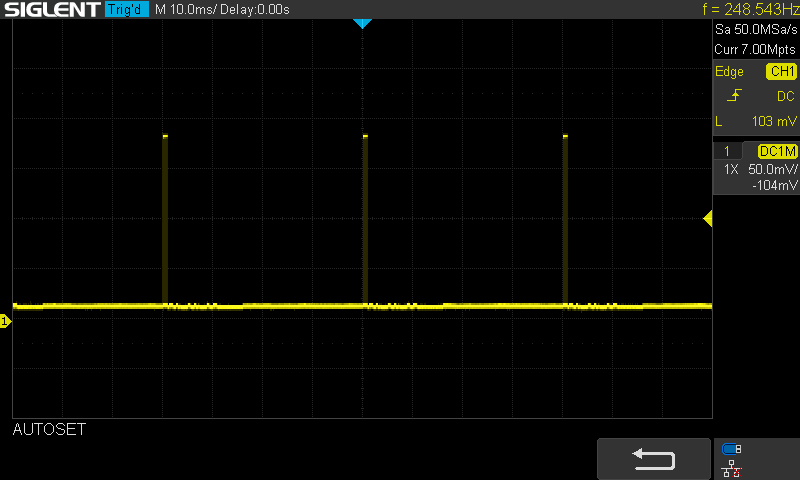
\includegraphics[width=133mm]{./Figures/rafagaCero.png}
	\caption{Rafaga de adquisiciones en el grado 0 de la senoide de referencia.}
	\label{fig:rafagaCero}
\end{figure}

\vspace{5mm}

En la figura \ref{fig:zeroCross} puede verse la comparación entre la senoide de referencia y la salida aislada ópticamente.

\vspace{5mm}

\begin{figure}[ht]
	\centering
	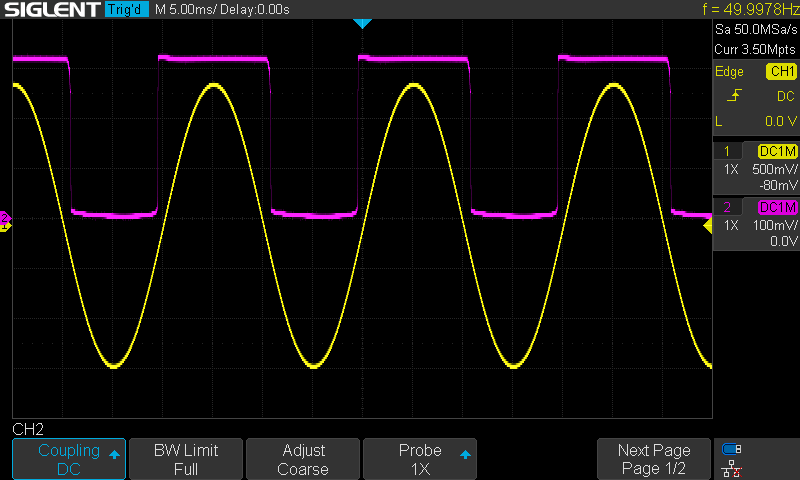
\includegraphics[width=133mm]{./Figures/zeroCross.png}
	\caption{Senoide de referencia y salida de detección de cruce por 0 optoacoplada.}
	\label{fig:zeroCross}
\end{figure}

\vspace{5mm}

Además de verificar disparos individuales configurados manualmente, se realizó un script en python con la librería Fygen \citep{fygenWeb:1} capaz de sintetizar un patrón de descargas parciales. Los datos utilizados provienen de archivos Matlab que fueron previamente generados en base a mediciones reales realizadas por el cliente.

En las figuras \ref{fig:corona1Original},\ref{fig:corona1Propia},\ref{fig:corona2Original} y \ref{fig:corona2Propia} pueden verse la comparativa entre el patrónes de DP generados por el cliente y su homonimo generado por el equipo en base a la misma secuencia de señales sintetizadas. Como difierencia se encuentra que la escala vertical del patron original se encuentra expresada en pC y la generada en mV debido al proceso de calibración que se realizó cuando las pruebas fueron tomadas. Como fue explicado al inicio de este capítulo la magnitud solo fue tomada como referencia por tratarse de un ensayo de fase.

\vspace{5mm}

\begin{figure}[htp] 
    \centering
    \subfloat[Corona original.]{%
        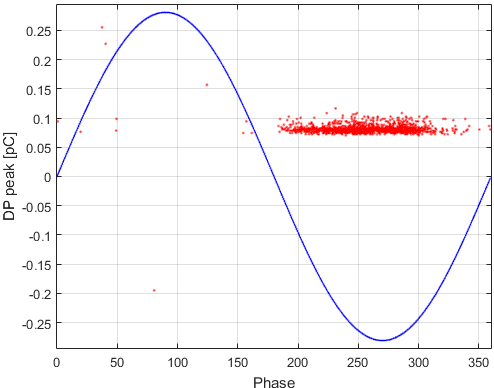
\includegraphics[width=0.46\textwidth]{./Figures/corona1Original.png}%
        \label{fig:corona1Original}%
        }%
    \hfill%
    \subfloat[Corona sintetizada.]{%
        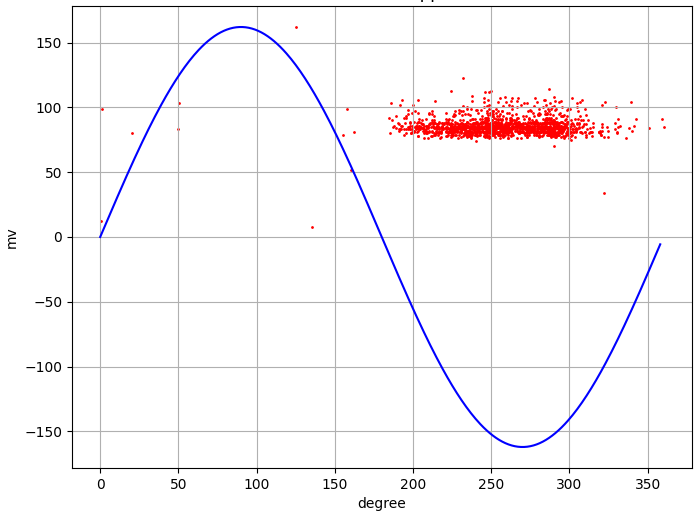
\includegraphics[width=0.5\textwidth]{./Figures/corona1Propia.png}%
        \label{fig:corona1Propia}%
        }%
    \caption{Comparación entre un patrón original y un patrón sintetizado.}
\end{figure}

\vspace{5mm}

\begin{figure}[htp] 
    \centering
    \subfloat[Corona original.]{%
        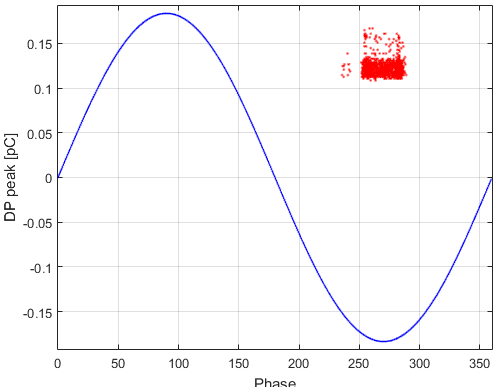
\includegraphics[width=0.475\textwidth]{./Figures/corona2Original.png}%
        \label{fig:corona2Original}%
        }%
    \hfill%
    \subfloat[Corona sintetizada.]{%
        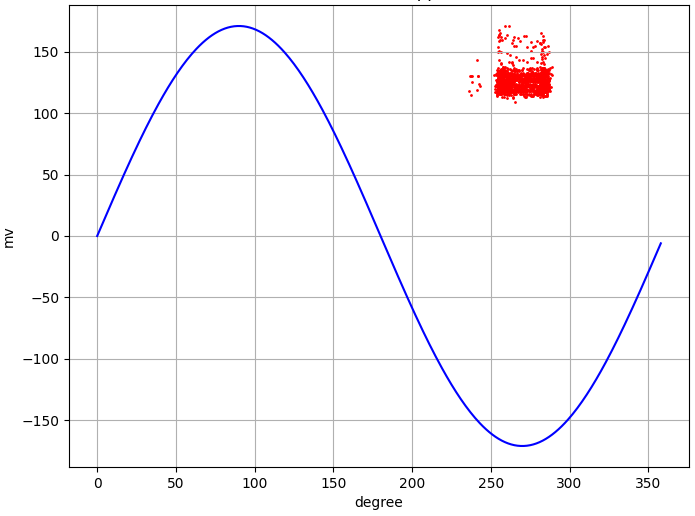
\includegraphics[width=0.5\textwidth]{./Figures/corona2Propia.png}%
        \label{fig:corona2Propia}%
        }%
    \caption{Comparación entre un patrón original y un patrón sintetizado.}
\end{figure}


\section{Tiempos de procesamiento}
Los ensayos de tiempo de procesamiento se realizaron utilizando un osciloscopio y un pin de salida de la placa \enquote{LPC link2} como marcador del estado interno del procesador. Durante este ensayo se buscó cuantificar el tiempo requerido por el procesador para realizar los distintos procesamientos. 

La operatoria de procesamiento se ejecuta al finalizar la adquisición de un bloque de memoria. Durante la misma se recorren los \textit{slots} en búsqueda del valor máximo absoluto, una vez encontrado se calcula la fase de la senoide de referencia que pertenece al mismo y se guarda en memoria RAM. Los resultados demuestran que para ejecutar este proceso sobre un banco de 16384 muestras, figura \ref{fig:tiempoSavePatron}, es necesario un tiempo de 5,5 mS. Esto equivale a 99° de desplazamiento angular de la senoide de referencia. 

Si el proceso es finalizado antes de comenzar un nuevo semiciclo el procesador puede rearmarse y continuar, de lo contrario deberá dejar un ciclo muerto.

\vspace{5mm}

\begin{figure}[ht]
	\centering
	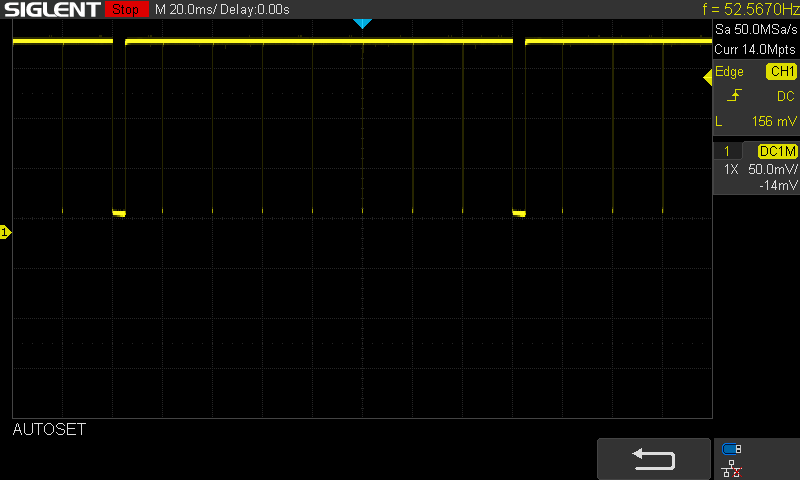
\includegraphics[width=133mm]{./Figures/tiempoSavePatron.png}
	\caption{Tiempo necesario para procesar 8 slots de memoria de 2048 muestras y obtener sus valores máximos absolutos con sus respectivas fases.}
	\label{fig:tiempoSavePatron}
\end{figure}

\vspace{5mm}

\section{Tiempos de almacenado}

Los ensayos de almacenamiento se realizaron con el fin de determinar cuánto tiempo requiere el procesador para almacenar el total de la adquisición en el soporte flash USB. Al igual que el procesamiento este proceso se realiza al completar un banco de memoria, por lo que se efectúan rafagas de escritura de 32 kB. Junto con el volcado de memoria se efectúa el proceso de búsqueda de pico y fase descripto en el ensayo de procesamiento. 

El tiempo requerido para realizar un vuelco de memoria y su procesamiento es de 16 mS, figura \ref{fig:tiempoSaveAll} , esto es igual a 288° de desplazamiento angular sobre la senoide de referencia. Al igual que en el proceso de procesamiento el sistema podrá rearmarse si finaliza antes del inicio de un nuevo periodo, de lo contrario deberá dejar un ciclo muerto.

\begin{figure}[ht]
	\centering
	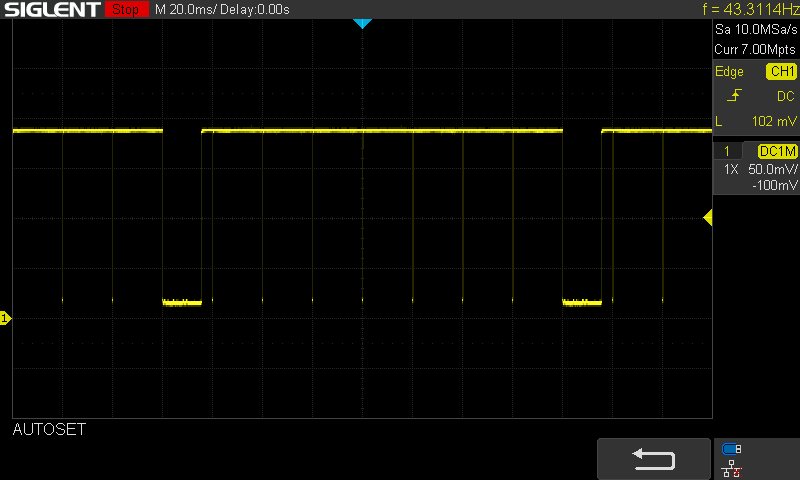
\includegraphics[width=133mm]{./Figures/tiempoSaveAll.png}
	\caption{Tiempo necesario para procesar 8 slots de memoria de 2048 muestras, obtener sus valores máximos absolutos con sus respectivas fases y almacenarlo en la unidad flash USB.}
	\label{fig:tiempoSaveAll}
\end{figure}

\newpage

\section{Pruebas en campo}
Debido a la pandemia global COVID-19 no fue posible realizar pruebas en campo ni en el laboratorio situado en la Universidad Tecnológica Nacional Regional General Pacheco. Dichos ensayos están pendientes a ser realizados cuando se tenga permiso de acceso al laboratorio.